\documentclass[10pt]{article}
\usepackage{preamble}
\usepackage[style=authoryear,natbib=true,uniquename=false,uniquelist=false]{biblatex}  % biber
\addbibresource{references.bib}

\newcommand{\hblee}[1]{{\it \color{cyan} #1}}

\title{
    Parameterizing the genetic architecture under apparent stabilizing selection
}

\author[1]{Hanbin Lee}
\author[1]{Jonathan Terhorst}

\affil[1]{Department of Statistics, University of Michigan, Ann Arbor, MI, 48109, USA}
\affil[$\dagger$]{\small These authors contributed equally}
\affil[$*$]{Correspondence to \texttt{hblee@umich.edu}}

\date{\today}

% Responses to reviews
%\input{review-response-commands}
% set this to show line numbers and include responses to reviews or not
%\newif\ifreviewresponses
%\reviewresponsestrue  % include them
% \reviewresponsesfalse  % don't include them
%\newcommand{\responsefile}{review-responses}  % name of the review responses file

\begin{document}

\maketitle

\begin{abstract}
    The effect sizes of trait-associated variants exhibit across many traits a common pattern of the magnitude decreasing as a function of minor allele frequency.
    This is assumed to be the result of negative selection where natural selection acts stronger against large effect variants, dragging their frequency downwards.
    To account for this phenomenon, it is common to model the variance of the effect to be inversely proportional to heterozygosity, namely the $\alpha$-model.
    Although the $\alpha$-model captures the inverse relationship of effect size and minor allele frequency to some extent,
    the modeling choice is arbitrary and lacks a population genetic foundation.
    To this end, we derive an alternative to the $\alpha$-model to address the frequency-dependent pattern of effect sizes from an \emph{apparent stabilizing selection} framework, whereby a focal trait is subject to selection indirectly due to a correlated trait experiencing stabilizing selection.
    Our new formula consists of three interpretable parameters, namely the mutational variance, stabilizing selection intensity, and genetic correlation.
    Furthermore, the new model can be conveniently estimated by the popular restricted maximum likelihood estimator and produces more accurate genetic prediction compared to the $\alpha$-model as we demonstrate in simulations.
\end{abstract}

\vspace{1em} 
\noindent \textbf{Keywords:} stabilizing selection; polygenic trait, statistical genetics

\section{Introduction}

% opening
With the rapid expansion of massive genomic datasets,
a tremendous amount of genetic variants associated to complex traits have been discovered through genome-wide association studies (GWAS) [cite].
Beyond identifying trait-associated loci, recent works have developed methods to aggregate signals under the statistical significance threshold.
These methods have been used for various purposes including, but not limited to,
heritability estimation, functional characterization, and natural selection detection [cite].
At the heart of these methods lies a formula that describes the magnitude of variant effect sizes as a function of minor allele frequency (MAF), linkage disequilibrium (LD), and functional annotations among many others [cite].
Such a formula describes how genetic variants contribute to trait genetics, hence the term \emph{genetic architecture}.

% frequency-dependence and alpha-model
A universally observed pattern in genetic architecture is that rare variants with lower frequencies tend to have larger effect sizes compared to the common variants of higher frequencies,
which is also called as frequency-dependence [cite].
This is usually understood in the context of negative selection where large effect variants are more likely to be removed from the population than small effect variants.
A common modelling choice is the $\alpha$-model where the variance of the effect size is inversely proportional to the power $\alpha$ of heterozygosity.
This model first appeared in the setting of estimating genetic relatedness matrices from single nucleotide polymorphism (SNP) markers and has later been extended to explicitly detect negative selection [cite].
Nevertheless, it is largely based on statistical curve-fitting and no population genetic model has yet been discovered to back this model.
Indeed, recent studies suggest leveraging population genetic theory to derive a more principled model instead of relying on statistical heuristics.

% paragraph on Simons et al. and its derivativs
Stabilizing selection has been adopted widely as means to explain complex trait variation [cite].
The seminal work of [Simons 2018, cite] has introduced the machinery of stabilizing selection to the GWAS literature.
They considered a multi-dimensional model of stabilizing selection and derived a distribution of a effect sizes conditioned on the effective selection coefficient.
As the frequency and effect sizes are correlated through the selection coefficient, 
conditioning removes the correlation between them, thereby simplifying the theory significantly.
From this simplification, one can predict the distribution of effect sizes as a function of heritability and target size [Simons 2025, cite].
Nevertheless, this framework focuses more on the selection coefficient instead of frequency, so the frequency-dependent architecture is not explicitly stated.
One might say that the effective selection coefficient replaces the role of variant frequency in this framework.

% apparent stabilizing selection
In this work, we consider an alternative framework of \emph{apparent stabilizing selection}.
A trait under apparent stabilizing selection may not be directly under selection but is correlated to a trait that is. 
This framework is well-suited for our problem as the true measure of fitness is practically unobservable.
There are three key parameters in our model: the intensity of stabilizing selection, 
and the variance and the genetic correlation of allelic substitution effect.
These three parameters provides a concise formula on how the variant effect size depend on allele frequency.
From a theoretical standpoint, the formula reveals an interpretable parameterization of the frequency-dependent genetic architecture and naturally incorporates the sample frequency instead of the unobservable population frequency.
Furthermore, the variance does not diverge to infinity as the frequency approaches zero like the $\alpha$-model.
Practically speaking, these parameters can be estimated using existing estimators such as the restricted maximum likelihood (REML), 
thereby allowing existing applications of linear mixed models, such as genetic prediction through best linear unbiased prediction (BLUP), to be used.




\section{Theory and model}

\subsection{The general framework}

\begin{table}[htpb]
    \centering
    \caption{Key mathematical notations}
    \label{tab:notation}
    \vspace{0.5em}
    \begin{tabular}{ll}
        \hline
        Symbol & Description \\
        \hline
        $y, z$ & Observed trait ($y$) and unobserved fitness-determining trait ($z$) \\
        $G$ & Genotype matrix \\
        $\alpha, \beta$ & Additive effect sizes of variants on fitness and observed trait \\
        $\veps, \delta$ & Non-genetic environmental components for $y$ and $z$ \\
        $\sigma_a^2, \sigma_b^2$ & Mutational variances of fitness and trait effect sizes \\
        $\rho_{ab}$ & Mutational correlation between fitness and trait \\
        $p_j, \hp_j$ & Population and sample minor allele frequency of locus $j$ \\
        $V_S$ & Variance of the stabilizing selection fitness landscape \\
        $W_S$ & Population-scaled selection parameter variance ($W_S = V_S / 2N$) \\
        $\seff(x)$ & Marginal selection coefficient at population allele frequency $x$ \\
        $N, \mu$ & Diploid population size and mutation rate \\
        $\theta$ & Population-scaled mutation rate ($\theta = 4N\mu$) \\
        $\pinf(x \mid \alpha)$ & Equilibrium density of allele frequency $x$ with fitness effect $\alpha$ \\
        \hline
    \end{tabular}
\end{table}
We consider an observed trait $y$ and an unobserved trait $z$ where the latter determines the fitness of an individual.
We assume an \emph{additive model} whereby both $y$ and $z$ are weighted sums of genotypes [cite].
\begin{gather}
    \begin{gathered}
        y_i = G_i\beta + \veps \\
        z_i = G_i\alpha + \delta
    \end{gathered}
\end{gather}
We assume the non-genetic component $\veps$ and $\delta$ to be normally distributed.
More generally, we may write the above relationship in terms of conditional probability
\begin{gather} \label{eq:trait_and_fitness}
    \begin{gathered}
        y_i \sim p(y_i \mid G_i, \beta) \\
        z_i \sim p(z_i \mid G_i, \alpha)
    \end{gathered}
\end{gather}
which means that $y$ and $z$'s distributions are determined by $G$ and the coefficients $\alpha, \beta$.

The key evolutionary consideration is the distribution of $G$ given $\alpha$ and $\beta$.
Its distribution is determined by two factors.
First, the samples are obtained from the population, then the population itself is evolving over time.
If we write the state of the population as $P_t$,
we can express $p(G \mid \alpha, \beta)$ as
\begin{align} \label{eq:definetti}
    \begin{aligned}
        p(G_i \mid \alpha, \beta) &=
        \int p(G_i \mid \alpha, \beta ,P_t)
        \cdot p(P_t \mid \alpha, \beta) dP_t \\
        &=
        \int p(G_i \mid P_t)
        \cdot p(P_t \mid \alpha, \beta) dP_t \\
        &=
        \int \underbrace{p(G_i \mid P_t)}_{\text{Sampling}}
        \cdot \underbrace{p(P_t \mid \alpha)}_{\text{Evolution}} dP_t
    \end{aligned}
\end{align}
Here, $p(G \mid \alpha, \beta, P_t) = p(G \mid P_t)$ because once the population state $P_t$ is given, the distribution of $G$ is entirely determined by the study's sampling scheme.
For instance, one can randomly sample genomes from the population with replacement.
The second simplification $P(P_t \mid \alpha, \beta) = P(P_t \mid \alpha)$ comes from the fact that $z$ determines the fitness through equation~\ref{eq:trait_and_fitness}.
As long as $\alpha$ is given, the evolution does not depend on $\beta$.

Finally, the distributions of $\alpha$ and $\beta$ have to be considered.
There are many loci in the genome, but only a fraction of them are segregating in the population.
Mutation chooses randomly from these loci that ultimately appears to be the variants in the observed dataset.
Furthermore, if the mutation rate is small enough, this process is effectively a \emph{sampling with replacement} scheme corresponding to the \emph{infinite-alleles} or the \emph{infinite-sites} assumption.
This argument first appeared in [cite, Kimura] as the continuum-of-alleles (CoA) model in the infinite-alleles context.
Hence, the distribution of $\alpha$ and $\beta$ in this paper refers to the random selection of effect sizes driven by mutation hitting random loci on the genome.
To simplify computations,
we assume normality
\begin{gather} \label{eq:coa}
\begin{pmatrix}
        \alpha_j \\
        \beta_j
    \end{pmatrix}
    \sim
    N\left(
    \begin{bmatrix}
        0 \\
        0
    \end{bmatrix}
    , 
    \begin{pmatrix}
        \sigma_{a,j}^2 & \rho_{ab,j}\sigma_{a,j}\sigma_{b,j} \\
        \rho_{ab,j} \sigma_{a,j} \sigma_{b,j} & \sigma_{b,j}^2
    \end{pmatrix} 
    \right)
\end{gather}
following the works of [cite, Lande].

\subsection{Connection to mixed-effects models}

Genomic mixed-effects models mainly consider the conditional distribution of $y$ given $G$.
Accordingly, the variance decomposition of the trait is
\begin{align}
    \begin{aligned}
    \var{y \mid G} &= \var{G\beta + \veps \mid G} \\
    &= G\var{\beta \mid G}G^T + \var{\veps \mid G} \\
    &= G\var{\beta \mid G}G^T + \var{\veps} 
    \quad
    (\because G \indep \veps) \\
    &= G \Sigma_\beta G^T + \var{\veps}
    \end{aligned}
\end{align}
where $\Sigma_\beta = \var{\beta \mid G}$.
A common model choice is the $\alpha$-model
\begin{align}
    \begin{aligned}
        \Sigma_\beta = \textrm{diag}
        \left( 
        \frac{h^2}{M } \cdot \frac{1}{[p_j(1-p_j)]^\alpha}
        \right) 
    \end{aligned} 
\end{align}
where $M$ is the number of variants and $h^2$ is a positive constant often referred to as the SNP-heritability.

In practice, we only have the sample frequency $\hp_j$ instead of $p_j$, so the estimate
\begin{align} \label{eq:alpha}
    \begin{aligned}
        \widehat{\Sigma}_{\beta} = \textrm{diag}
        \left( 
        \frac{h^2}{M } \cdot \frac{1}{[\hp_j(1-\hp_j)]^\alpha}
        \right) 
    \end{aligned}
\end{align}
replaces $\Sigma_\beta$.
The $\alpha=1$ case is the genome-wide complex trait analysis (GCTA) model [cite, Yang].
Together with $G$, $G \widehat{\Sigma}_{\beta}G^T$ is a genomic estimate of genetic relatedness, called the genomic genetic relatedness matrix (GRM) [cite].
For a more comprehensive review of different choices of $\Sigma_\beta$, see [cite].

Despite its empirical success [cite], 
equation~\ref{eq:alpha} and its variants have several shortcomings.
In particular, the choice of $\Sigma_\beta = \var{\beta \mid G}$ was assumed making its parameters $h^2$ and $\alpha$ merely tuning parameters without an explicit biological interpretation, although heuristic arguments exist.
For instance, a positive $\alpha$ partially captures the inverse relationship between minor allele frequency and effect size [cite].
A notable pathological behavior is that $[p_j(1-p_j)]^{-\alpha}$ diverges to infinity as $p_j$ approaches zero, requiring heuristic GRM partitioning over multiple MAF bins [cite, Wainschtein].
It is also unclear if the sample frequency $\hp_j$ can replace the true frequency $p_j$, especially in rare variants.

Our framework offers a principled solution to the aforementioned issues.
From equations~\ref{eq:definetti} and~\ref{eq:coa}, we can determine $p(\beta \mid G)$ using the Bayes formula.
\begin{align} \label{eq:goal1}
    \begin{aligned}
    p(\beta \mid G) & \ \propto \
    p(G \mid \beta) \cdot p(\beta) \\
    &= \int p(G \mid \alpha, \beta) \cdot p(\alpha \mid \beta) d\alpha \cdot p(\beta) \\
    &= \int p(G \mid \alpha) \cdot p(\alpha \mid \beta) d\alpha \cdot p(\beta)
    \end{aligned}
\end{align}
and compute
\begin{align} \label{eq:goal2}
    \var{\beta \mid G} = \int \beta^2 p(\beta \mid G) d\beta.
\end{align}
What is left is to find the appropriate formula of $p(\beta \mid G)$ to complete the formula.
Since $p(G\mid\alpha)$ in equation~\ref{eq:goal1} contains evolutionary information,
the final formula will be naturally expressed in terms of evolutionary parameters of the system.

\subsection{Diffusion approximation for stabilizing selection}

We assume that an individual's fitness is given by
\begin{align}
    \exp \left(
        -\frac{z^2}{2V_S} 
    \right)
\end{align}
where $z$ is the trait value subject to stabilizing selection and $V_S$ controls selection intensity.
The marginal selection coefficient $\seff$ is given by
\begin{align} \label{eq:seff}
    \seff(x) = \left(x-\frac{1}{2}\right)\frac{\alpha^2}{V_S}
\end{align}
for a biallelic loci of frequency $x$ and effect size $\alpha$ \citep{Robertson1956againstextreme,Lande1976phenoevolution,Simons2018popgeninterpretation, Negm2024longrangeld}.
In a panmictic diploid population of size $N$,
the diffusion approximation corresponding to equation~\ref{eq:seff} is
\begin{align} \label{eq:wf_diffusion_raw}
    \begin{aligned}
    dX_t &= (\seff(X_t)X_t(1-X_t) + \mu(1-2X_t))dt + \sqrt{\frac{X_t(1-X_t)}{2N}}dB_t \\
    &= \left[ X_t(1-X_t)\left(X_t-\frac{1}{2}\right)\frac{\alpha^2}{V_S}
    + \mu(1-2X_t) 
    \right] 
    dt + \sqrt{\frac{X_t(1-X_t)}{2N}}dB_t
    \end{aligned}
\end{align}
where $B_t$ is the Brownian motion.
We choose to measure $V_S$ in units of $2N$,
so we write $V_S = 2N \cdot W_S$.
Accordingly, we keep $\theta = 4N\mu$.
By scaling equation~\ref{eq:wf_diffusion_raw} by the $2N$ factor,
we obtain
\begin{align} \label{eq:wf_diffusion_scaled}
    dX_t = \left[
    X_t(1-X_t)\left(X_t-\frac{1}{2}\right)\frac{\alpha^2}{W_S} 
    + \frac{1}{2}\theta(1-2X_t)
    \right] 
    dt + \sqrt{X_t(1-X_t)}dB_t   
\end{align}
with the forward Kolmogorov equation given by
\begin{align} \label{eq:fwd_kolmogorov_scaled}
    \begin{aligned}
     \pard{p(x,t;\alpha)}{t} 
     =& -\pard{}{x} 
     \left[
     \left(
        x(1-x)\left(x-\frac{1}{2}\right)
        \frac{\alpha^2}{W_S}
        + \frac{1}{2}\theta(1-2X_t)
        \right)
        p(x,t;\alpha)
     \right] \\
     &+\frac{1}{2} \pard[2]{}{x}[x(1-x)p(x,t;\alpha)].
     \end{aligned}
\end{align}

We'll make use of the stationary density $p(x,t;\alpha)$ of equation~\ref{eq:fwd_kolmogorov_scaled}.
This can be obtained by setting the left-hand side to zero, meaning that the density does not change with respect to $t$ \citep{Ewens2004mathpopgen}.
\begin{align} \label{eq:stat_dist}
     p_{\infty}(x;\alpha) = C(\alpha)^{-1} \cdot
     x^{\theta-1}(1-x)^{\theta-1} 
     \exp\left[-\frac{\alpha^2}{W_S}x(1-x) \right]
\end{align}
with the normalizing constant 
\begin{align} \label{eq:norm_const}
    C(\alpha) = \int_0^1 x^{\theta-1}(1-x)^{\theta-1} 
    \exp\left[-\frac{\alpha^2}{W_s}x(1-x) \right] dx = B(\theta, \theta) 
    \cdot {_1F_1} \left(
    \theta; \theta + \frac{1}{2}; -\frac{\alpha_j^2}{4W_S}
    \right)
\end{align}
where $_1F_1(a;b;z)$ is the Kummer's hypergeometric function.
Fortunately, $_1F_1(a;b;z) = 1 + \mathcal{O}(a)$, so we can ignore the factor as $\theta \rightarrow 0$.

\subsection{Deriving the approximate genetic architecture}

We now return to deriving $p(\beta \mid G)$.
The first approximation we apply to the expression is
\begin{align} \label{eq:mean_field}
    p(\beta \mid G) = \prod_j p(\beta_j \mid G_j)
\end{align}
and we expand $p(\beta_j \mid G_j)\ \propto \ p(G_j \mid \beta_j) \cdot p(\beta_j)$ with the results from the diffusion approximation.

Let $\hp_j$ be the sample frequency computed from $G_j$. Then,
\begin{align} \label{eq:xll}
        p(G_j \mid \beta_j) 
        = p(\hp_j \mid \beta_j) 
        = \int_0^1 
        \underbrace{\binom{2n}{k_j} x_j^{k_j}(1-x_j)^{2n-k_j}}_{\text{Binomial sampling}}
        \ \cdot \ 
        \underbrace{\vphantom{\binom{1}{k_j}}\pinf(x_j \mid \beta_j)}_{\text{Evolution}} dx_j
\end{align}
where $k_j$ is the number of the minor allele $j$ in the sample and $\pinf(x_j \mid \beta_j)$ is the equilibrium distribution of the population frequency $x_j$.
One can see that this expression resembles the site frequency spectrum (SFS) [cite].

We substitute 
\begin{align}
    \pinf(x_j \mid \beta_j) 
        =
        \int \pinf(x_j \mid \alpha_j, \beta_j) \cdot p(\alpha_j \mid \beta_j) d\alpha_j 
        = \int \pinf(x_j \mid \alpha_j) \cdot p(\alpha_j \mid \beta_j) d\alpha_j 
\end{align}
to equation~\ref{eq:xll} and swap integrations to get
\begin{align} \label{eq:swapped}
    \begin{aligned}
    p(G_j \mid \beta_j) &=
    \int_0^1 \int 
    \binom{2n}{k_j} x_j^{k_j}(1-x_j)^{2n-k_j}
    \pinf(x_j \mid \alpha_j) p(\alpha_j \mid \beta_j) d\alpha_j dx_j \\
    &= \int \int_0^1
    \binom{2n}{k_j} x_j^{k_j}(1-x_j)^{2n-k_j}
    \pinf(x_j \mid \alpha_j) p(\alpha_j \mid \beta_j) dx_j d\alpha_j  \\
    &= \int p(\alpha_j \mid \beta_j)\int_0^1
    \binom{2n}{k_j} x_j^{k_j}(1-x_j)^{2n-k_j}
    \pinf(x_j \mid \alpha_j)  dx_j d\alpha_j. 
    \end{aligned}
\end{align}

Although the inner integral looks complicated at first sight, 
large sample asymptotics, namely $n \rightarrow \infty$ and $k_j/2n \rightarrow \hp_j$, greatly simplifies the integration.
Due to the fact that the beta-binomial distribution collapses to a degenerate form with increasing sample size,
\begin{align} \label{eq:beta_to_dirac}
    \begin{aligned}
        & \int_0^1 
        \binom{2n}{k_j} 
        x_j^{k_j}(1-x_j)^{2n-k_j}
        \pinf(x_j \mid \alpha_j) 
        dx_j \\
        & \ \propto \ \int_0^1   
        \binom{2n}{k_j} 
        x_j^{k_j}(1-x_j)^{2n-k_j}
        x_j^{\theta-1}(1-x_j)^{\theta-1}
        \exp\left[-\frac{\alpha_j^2}{W_S}x_j(1-x_j) \right]dx_j \\
        &\ \propto \ \exp\left[-\frac{\alpha_j^2}{W_S}\hp_j(1-\hp_j) \right]
    \end{aligned}
\end{align}
where the integration turned into a substitution $x_j \leftarrow \hp_j$.
Observe that the sample frequency $\hp_j$ naturally appears in the formula.
Next, we put equation~\ref{eq:beta_to_dirac} back into equation~\ref{eq:swapped} to get
\begin{align}
    \begin{aligned}
        p(G_j \mid \beta_j) 
        &\ \propto \
        \int p(\alpha_j \mid \beta_j) \cdot 
        \exp\left[-\frac{\alpha_j^2}{W_S}\hp_j(1-\hp_j) \right] d\alpha_j \\
        & \ \propto \ \int
        \exp \left[ -\frac{\left( \alpha_j - \rho_{ab,j} \frac{\sigma_{a,j}}{\sigma_{b,j}} \beta_j \right)^2}{2 \sigma_{a,j}^2 (1 - \rho_{ab,j}^2)} \right]
        \exp\left[-\frac{\alpha_j^2}{W_S}\hp_j(1-\hp_j) \right] d\alpha_j 
        \\
        & \ \propto \
        \exp \left[ -\frac{\hat{p}_j(1 - \hat{p}_j) \rho_{ab,j}^2 \frac{\sigma_{a,j}^2}{\sigma_{b,j}^2} \beta_j^2}{W_s + 2\sigma_{a,j}^2(1 - \rho_{ab,j}^2)\hat{p}_j(1 - \hat{p}_j)} \right].
    \end{aligned}
\end{align}

At last, we arrive at the formula for $p(\beta_j \mid G_j)$ by
\begin{align}
    p(\beta_j \mid G_j) &\ \propto \ 
    \exp \left[ -\frac{\hat{p}_j(1 - \hat{p}_j) \rho_{ab,j}^2 \frac{\sigma_{a,j}^2}{\sigma_{b,j}^2} \beta_j^2}{W_s + 2\sigma_{a,j}^2(1 - \rho_{ab,j}^2)\hat{p}_j(1 - \hat{p}_j)} \right] \cdot p(\beta_j), 
\end{align}
a Gaussian density which has the variance of
\begin{align} \label{eq:beta_cond_var}
    \E{\beta_j^2 \mid G_j} = \E{\beta_j^2 \mid \hp_j} = 
    \sigma_{b,j}^2 \cdot 
    \left[
        \frac{
            1 + (1-\rho_{ab,j}^2) \cdot 2\frac{\sigma_{a,j}^2}{W_S} \hp_j(1-\hp_j)}{
            1 + 2\frac{\sigma_{a,j}^2}{W_S} \hp_j(1-\hp_j) 
        }
    \right]
\end{align}
with effectively three parameters $\sigma_b^2$, $\sigma_a^2 / W_S$, and $\rho$.
Note that $W_S$ and $\sigma_a^2$ cannot be separately identified because the formula remains invariant with respect to a common scaling factor.

The formula has several important properties.
First, if the trait $y$ is uncorrelated with fitness $z$ ($\rho=0$), it reduces to $\sigma_b^2$ and has no dependence on the sample frequency $\hp_j$.
Secondly, it is always bounded above by $\sigma_b^2$, so does not diverge to infinity regardless of the value of $\hp_j$.
Nevertheless, it captures the negative correlation between $\hp_j$ and the magnitude of $\beta_j$.
Finally, it captures the intuition from earlier studies that the relative ratio of mutational variance $\sigma_{a,j}^2$ and selection width $W_S$ determines the system [cite, Hayward].

When majority of variants are small, equation~\ref{eq:beta_cond_var} carries an identification issue.
To see this,
\begin{align}
    \begin{aligned}
    \E{\beta_j^2 \mid \hp_j} &= 
         \sigma_{b,j}^2 \cdot 
    \left[
        \frac{
            1 + (1-\rho_{ab,j}^2) \cdot 2\frac{\sigma_{a,j}^2}{W_S} \hp_j(1-\hp_j)}{
            1 + 2\frac{\sigma_{a,j}^2}{W_S} \hp_j(1-\hp_j) 
        }
    \right]  \\
    &= \sigma_{b,j}^2 \cdot 
    \left[
    1 - 
    \rho_{ab,j}^2 \cdot 
        \frac{
             2\frac{\sigma_{a,j}^2}{W_S} \hp_j(1-\hp_j)}{
            1 + 2\frac{\sigma_{a,j}^2}{W_S} \hp_j(1-\hp_j) 
        }
    \right] \\
    &\approx \sigma_{b,j}^2 \cdot 
    \left[
    1 - 
             2\frac{\rho_{ab,j}^2\sigma_{a,j}^2}{W_S} \hp_j(1-\hp_j)
    \right]
    \end{aligned}
\end{align}
for small $\hp_j$.
Hence, we essentially have only two parameters: $\sigma_{b}^2$ and $\frac{\rho^2_{ab}\sigma_a^2}{W_S}$.

The above expression linearizes the formula, which we found to work poorly for estimation.
We found that the following parameterization obtained from matching first-order Taylor expansion works the best in practice.
\begin{align}
    \begin{aligned}
     \E{\beta_j^2 \mid \hp_j} &\approx
     \sigma_{b,j}^2 \cdot
     \frac{1}{1
     +2 \frac{\rho_{ab,j}^2\sigma_a^2}{W_S}\hp_j(1-\hp_j)}.
    \end{aligned} 
\end{align}

A more general relationship between $\alpha_j$ and $\beta_j$ can be obtained by the tower property
\begin{align}
    \begin{aligned}
        \E{\beta_j^2 \mid \hp_j}
        &= \E{\E{\beta_j^2 \mid \alpha_j} \mid \hp_j}
    \end{aligned}
\end{align}
which only requires $\E{\beta_j^2 \mid \alpha_j}$ instead of the full joint distribution.


\section{Simulation and empirical study}


\textcolor{red}{Everything above is hand-written. All below is GENAI. Curious how people manage to write meaningful stuffs using it. Only the numbers are correct and mostly rubbish.}

\subsection{SLiM simulation}
We conducted forward-time, individual-based simulations using the SLiM simulation framework to generate population genetic datasets under an infinite-sites quantitative trait model subject to stabilizing selection. Our foundational scenario simulated a panmictic demographic history with a constant diploid population size of $N=10{,}000$ individuals. To correctly capture the macro-level genetic architecture and linkage blocks, we simulated sequences scaled up to $L=10^6$ loci. Simulation parameters were appropriately scaled from a reference configuration ($L_{\text{ref}}=50{,}000$, $N_{\text{ref}}=10{,}000$) to the active genome sequence to maintain intended target architecture constraints. An aggregate reference mutation rate of $U_{\text{ref}} = 0.01$ yielded a per-locus mutation rate of $\mu = (U_{\text{ref}}/L) \times (N_{\text{ref}}/N) = 10^{-8}$, and the uniform per-generation recombination rate was scaled to $r = 10^{-3} \times (L_{\text{ref}}/L) = 5 \times 10^{-5}$.

The trait architecture was framed by a strictly additive genetic model without environmental variance ($V_E = 0$). Mutational effect sizes were drawn from a zero-centered Gaussian prior with an expected mutational variance $\sigma_a^2$. The fitness dynamics were governed by evaluating individuals' centered additive trait values against an optimizing Gaussian fitness landscape where the parameter $V_S$ dictates selection strength. Specifically, we assessed a systematic parameter grid of $50$ independent simulation replicates per configuration. We varied the population-scaled selection parameter $W_S = V_S / 2N \in \{0.5, 1.0, 2.0\}$ and the genetic variation scalar $\sigma_a^2 \in \{0.5, 1.0, 2.0\}$. All population paths underwent a preliminary burn-in period of $10N$ generations ($\approx 100{,}000$ generations) to reach equilibrium site frequency dynamics, followed by $40{,}000$ further generations simulating the active observational regime.


\subsection{Variance component estimation}

A major advantage of theoretically grounding the linear mixed model in population genetics is that the variance components become directly interpretable as evolutionary parameters. To evaluate our approach, we employed forward-time simulations of polygenic trait evolution under stabilizing selection using SLiM framework. We then fit the explicit frequency-dependent variance model via restricted maximum likelihood (REML) across a varying grid of true mutational variances ($\sigma_a^2$) and selection widths ($W_s$).

We emphasize that the parameterization primarily permits joint estimation of the genetic architecture through combinations like the ratio $\sigma_a^2 / W_s$. Figure~\ref{fig:blm_sigma2_a_over_ws} demonstrates that the model faithfully recovers the unbiased ratio $\sigma_a^2 / W_s$ with low empirical variance irrespective of the specific true $\sigma_a^2$ regime. Furthermore, Figure~\ref{fig:blm_sigma2_a} confirms that the individual mutational variance $\sigma_a^2$ itself is unbiasedly characterized throughout our experimental grid of true stabilizing selection strengths. Combined, these results empirically validate the diffusion approximation detailed in our theory.

\begin{figure}[htpb]
    \centering
    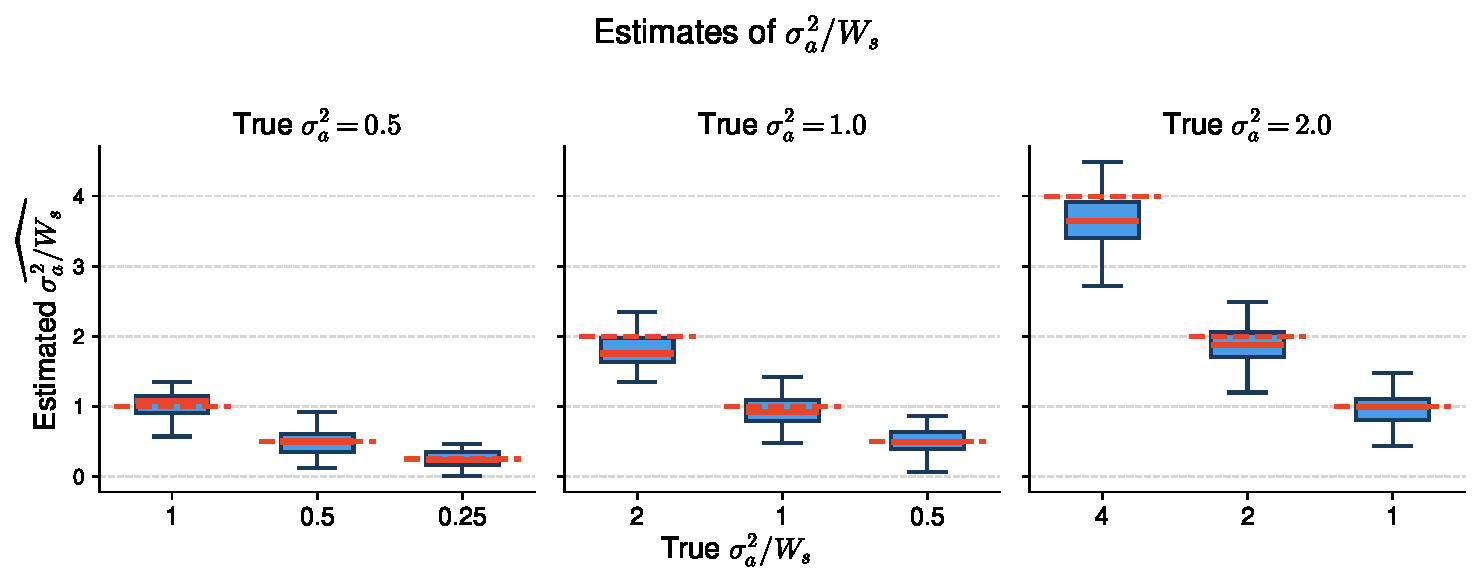
\includegraphics[width=\textwidth]{figs/blm_summary_sigma2_a_over_Ws.pdf}
    \caption{Recovery of the relative genetic architecture parameter. REML estimates of the ratio $\sigma_a^2 / W_s$ are presented across simulation replicates for varying underlying true configurations of stabilizing selection and variance.}
    \label{fig:blm_sigma2_a_over_ws}
\end{figure}

\begin{figure}[htpb]
    \centering
    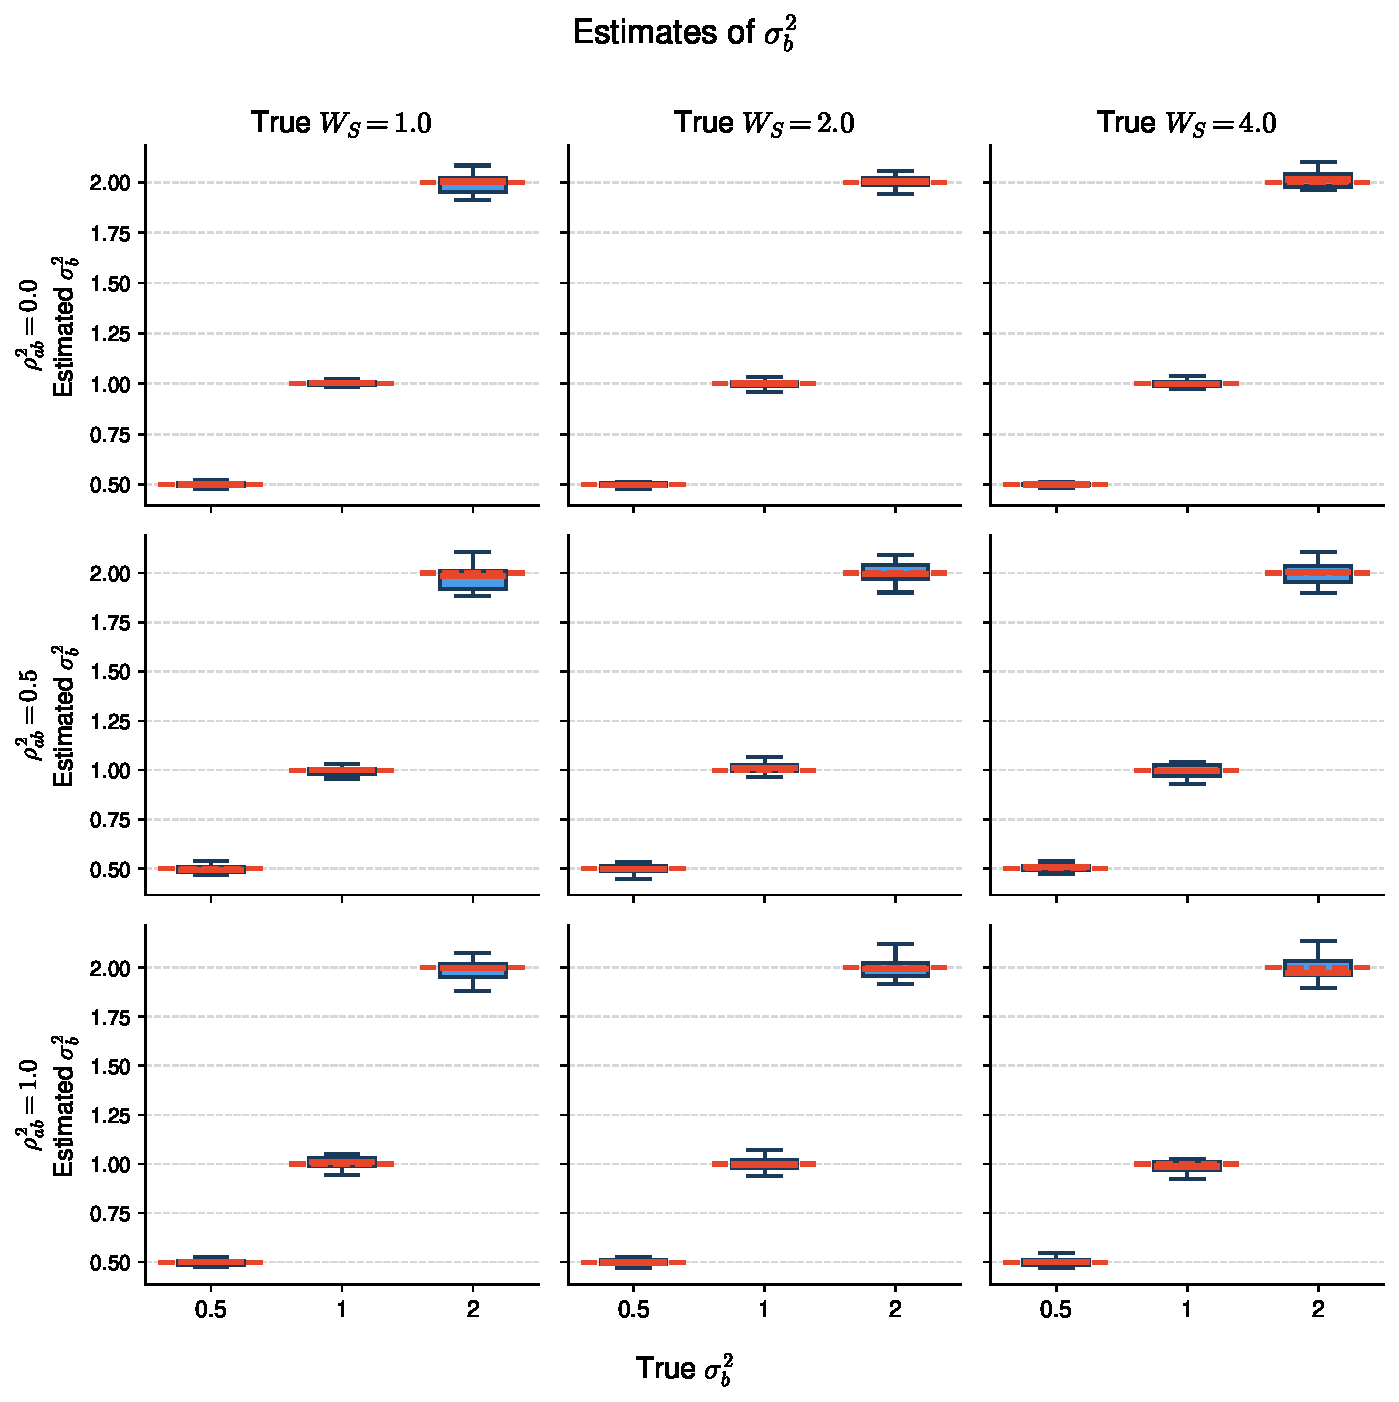
\includegraphics[width=\textwidth]{figs/blm_summary_sigma2_a.pdf}
    \caption{Unbiased recovery of the mutational variance parameter. REML estimates of $\sigma_a^2$ tightly match the theoretical expectations (dashed lines) independently across different selection regimes ($W_s \in \{0.5, 1.0, 2.0\}$).}
    \label{fig:blm_sigma2_a}
\end{figure}

\subsection{Genetic prediction}

To assess whether the evolutionary derivation leads to tangible benefits in practical inference tasks, we benchmarked the predictive performance of best linear unbiased prediction (BLUP). Both the stabilized evolutionary model (derived in the previous section) and the standard $\alpha$-model were evaluated across a grid of parameter scenarios. Specifically, we varied the mutational variance parameter $\sigma_a^2$ and the intrinsic phenotypic selection width $W_s$, controlling the architecture's susceptibility to genetic drift versus strong stabilizing selection.

Figure~\ref{fig:blup_prediction} presents the validation $R^2$ and correlation for the two models across independent simulation replicates. Our explicitly derived frequency-dependent architecture mitigates prediction errors associated with alleles subjected to strong selection where traditional $\alpha$-models systematically fail. As the intensity of selection increases relative to mutational variation (decreasing true $W_s$ and increasing $\sigma_a^2$), the baseline $\alpha$-model exhibits highly erratic, deteriorated predictive validation scores. Constrastingly, the theoretically grounded evolutionary architecture remains unbiased, preserving robust and tight predictive correlations and systematically outperforming the heuristic parameterization across all realistic regimes.

\begin{figure}[htpb]
    \centering
    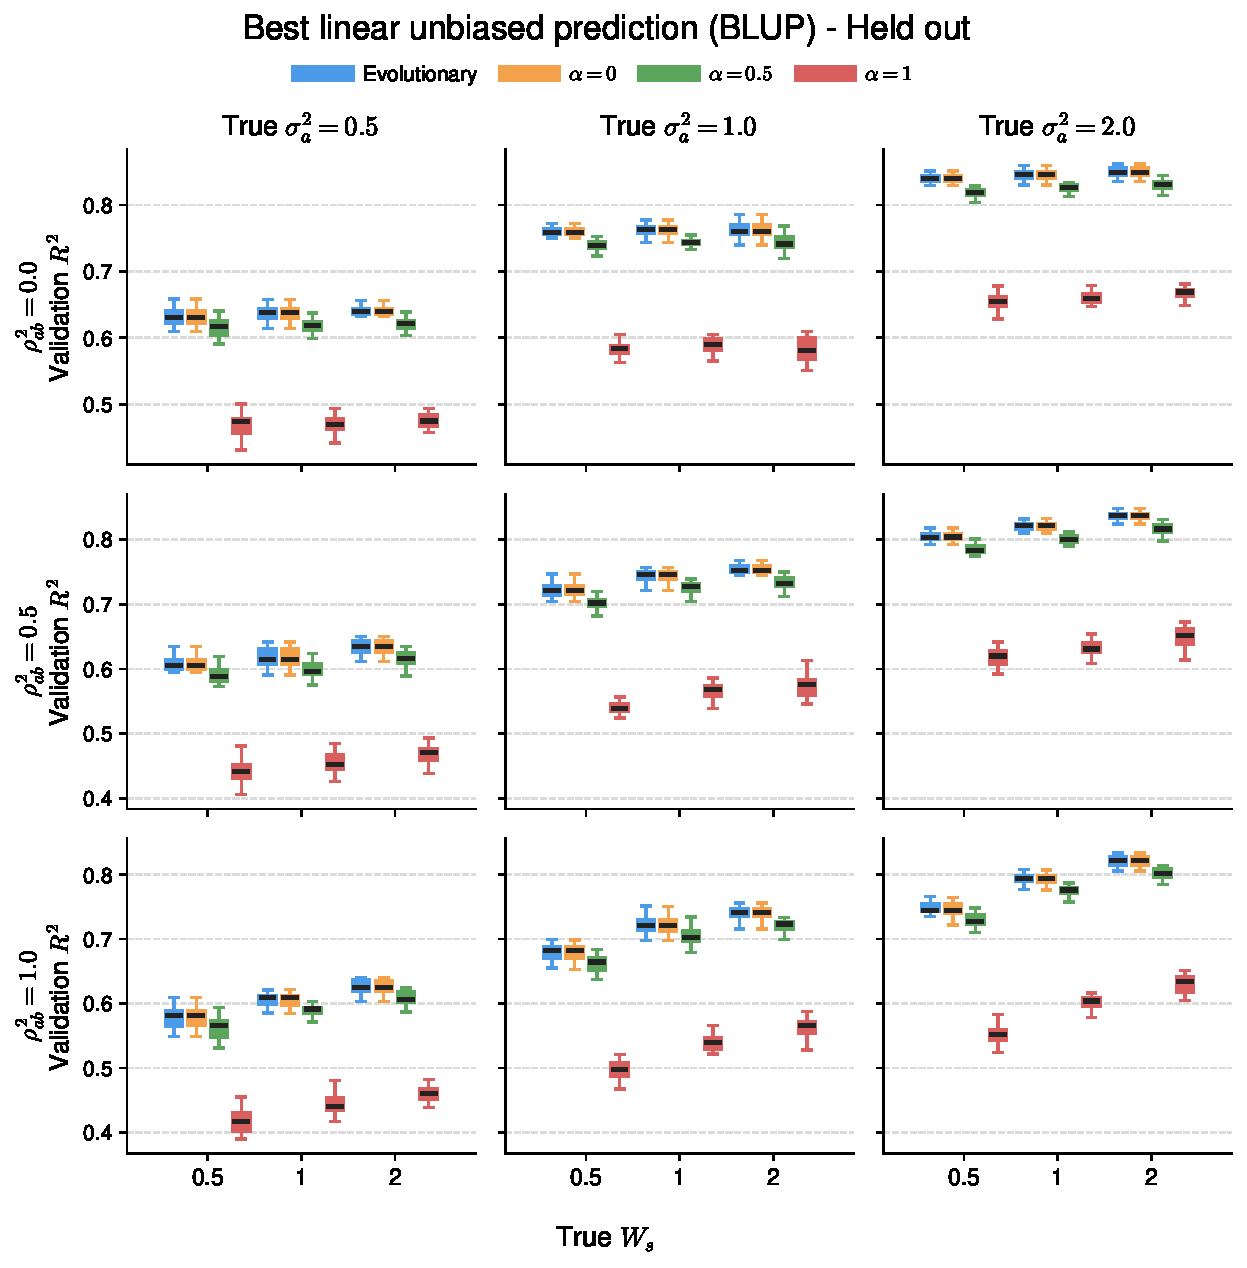
\includegraphics[width=\textwidth]{figs/blup_summary_prediction.pdf}
    \caption{Benchmark of genetic prediction performance. Validation $R^2$ and correlation across simulated replicates are shown for varying configurations of true $\sigma_a^2$ and selection parameter $W_s$. The evolutionary parameterization systematically outperforms the standard $\alpha$-model, particularly in regimes characterized by strong relative stabilizing selection ($W_s=0.5$).}
    \label{fig:blup_prediction}
\end{figure}


\section{Discussion}

We described how to deduce the genetic architecture of complex traits from the apparent stabilizing selection framework.
The resulting formula of variant effects describes the frequency-dependent architecture through evolutionarily informative parameters, overcoming the issues of earlier models based on statistical heuristics.
We further demonstrated that the model has practical utility due to easy fitting through the REML estimator that allows subsequent applications such as genetic prediction.
The simulations shows that the evolutionary approach is not only theoretically compelling, but also offers huge gains in genetic prediction compared to the heuristic models.

Our theoretical setup can be viewed






\newpage


\textcolor{red}{Everything below is scrible notes}




One can further consider the sample statistics under this model.
Suppose that we obtained $k$ derived allele copies out of $n$ samples.
Assume that $n \rightarrow \infty$ and $k/n \rightarrow \hp \in (0,1)$.
\begin{align} \label{eq:sample_freq_spectrum}
    \begin{aligned}
        &p(\text{$k$ out of $n$ copies}; \alpha) \approx p(\hp; \alpha)  \\
        &= \lim_{n,k \rightarrow \infty}
        \int_0^1 \binom{n}{k} x^{k} (1-x)^{n-k}
        C(\alpha)^{-1} \cdot
     x^{\theta-1}(1-x)^{\theta-1} 
     \exp\left[-\frac{\alpha^2}{W_s}x(1-x) \right] dx\\
     &= \lim_{n,k \rightarrow \infty} 
     C(\alpha)^{-1} \frac{1}{n+1}
     \frac{B(k+\theta, n-k + \theta)}{B(k+1,n-k+1)} \\
     &\,\cdot\int_0^1 \frac{1}{B(k+\theta,n-k+\theta)} x^{k+\theta-1}(1-x)^{n-k+\theta-1}
     \exp\left[-\frac{\alpha^2}{W_s}x(1-x)\right] dx \\
     &= \lim_{n,k \rightarrow \infty}
     C(\alpha)^{-1} \frac{1}{n+1}
     \frac{B(k+\theta, n-k + \theta)}{B(k+1,n-k+1)}
     \cdot \E[x \sim B(k+\theta,n-k+\theta)]{
        \exp\left(-\frac{\alpha^2}{W_s}x(1-x)\right)
     } \\
     &= C(\alpha)^{-1} \cdot 
     \exp\left[-\frac{\alpha^2}{W_s}\hp(1-\hp)\right]
     \cdot \lim_{n,k \rightarrow \infty} 
     \frac{1}{n+1}
     \frac{B(k+\theta, n-k + \theta)}{B(k+1,n-k+1)} \\
     &\approx C(\alpha)^{-1} \cdot 
     \exp\left[-\frac{\alpha^2}{W_s}\hp(1-\hp)\right]
     \cdot \mathcal{O}(n^{-1})
    \end{aligned}
\end{align}
giving the sample probability given the effect size $\alpha$.

\subsection{Modelling evolution in linear mixed models}
The sample frequency spectrum derived in equation~\ref{eq:sample_freq_spectrum} can be used in the context of linear mixed models.
Suppose that $\balpha \sim N(0, \sigma_a^2\bI)$ is the vector of effect sizes,
$\bG \in \real^{n \times p}$ is the genotype matrix, and $\bz \in \real^n$ is the vector of fitness.

The joint likelihood of $\bz$, $\bG$ and $\balpha$ is
\begin{align} \label{eq:joint_like_fitness}
    \begin{aligned}
        p(\bz, \bG, \balpha) &= p(\bz \mid \bG, \balpha)
        \cdot p(\bG \mid \balpha) 
        \cdot p(\balpha) \\
    \end{aligned}
\end{align}
with the negative logarithm being
\begin{align}
    \begin{aligned}
        - \log p (\bz, \bG, \balpha)
        &= - \log p(\bz \mid \bG, \balpha) - \log p(\bG \mid \balpha) - \log p (\balpha) \\
        &= \frac{n}{2}\log(\sigma_e^2) + \frac{1}{2\sigma_e^2}\norm{\by - \bG \balpha}_2^2 \\
        &+ \sum_{j=1}^pC(\alpha_j) + \frac{\hp_j(1-\hp_j)}{W_s} \alpha_j^2 \\
        &+ \frac{p}{2}\log(\sigma_a^2) + \frac{1}{2\sigma_a^2}\sum_{j=1}^p \alpha_j^2
    \end{aligned}
\end{align}
after discarding the constants.

We generally integrate over $\balpha$ to obtain the marginal likelihood $p(\bz, \bG)$ that serves as an optimization target,
but this is not analytically tractable due to $C(\alpha_j)$.
Hence, we focus on the second moment.
\begin{align}
    \begin{aligned}
        p(\alpha_j \mid \hp_j) 
        &\ \propto \ p(\hp_j \mid \alpha_j) \cdot p(\alpha_j) \\
        &= \cdots \\
        &= \frac{1}{ _1F_1\left(\theta; \theta+\frac{1}{2};-\frac{\alpha_j^2}{4W_S}\right)} 
        \cdot 
        \exp\left[
        -\alpha_j^2\left(
        \frac{\hp_j(1-\hp_j)}{W_S}
         + \frac{1}{2\sigma_a^2}
        \right)
        \right]
    \end{aligned} 
\end{align}
where $_1F_1(a;b;z)$ is the Kummer's hypergeometric function.
The second moment is 
\begin{align}
    \E{\alpha_j^2 \mid \hp_j} =
    \frac{1}{2\left( \frac{\hp_j(1-\hp_j)}{W_S} + \frac{1}{2\sigma_a^2} \right)} 
    + \frac{\theta}{4W_S \left( \frac{\hp_j(1-\hp_j)}{W_S} + \frac{1}{2\sigma_a^2} \right)^2}
\end{align}
accounting for the first order expansion of $_1F_1$.
\begin{align}
    _1 F_1(a;b;z) \approx 1 + \frac{a}{b}z + \mathcal{O}(z^2)
\end{align}

The genetic relatedenss matrix is
\begin{align}
    \bG \cdot 
    \begin{bmatrix}
        \E{\alpha_1^2 \mid \hp_j} & \cdots & 0 \\
        0 & \ddots & 0 \\
        0 & \cdots & \E{\alpha_p^2 \mid \hp_j}
    \end{bmatrix}
    \bG^T
\end{align}
which can be plugged into restricted maximum likelihood (REML).
Although common approaches derive REML from multivariate normal models,
the point estimate is consistent as long as the variance is correctly specified.

\subsection{Functional annotation as a proxy for fitness}
% have to mention pleiotropy

Let $\by$ and $\bbeta$ be the trait and the effect size of $\by$.
Then the likelihood similar to equation~\ref{eq:joint_like_fitness} is
\begin{align}
    \begin{aligned}
    p(\by, \bG, \bbeta) 
    &= 
    p(\by \mid \bG, \bbeta) \cdot p(\bG \mid \bbeta) \cdot p(\bbeta)  \\
    &= 
    p(\by \mid \bG, \bbeta) \cdot \int p(\bG, \balpha \mid \bbeta) d\balpha \cdot p(\bbeta)  \\
    &=
    p(\by \mid \bG, \bbeta) \cdot \int p(\bG, \mid \balpha ,\bbeta) p(\balpha \mid \bbeta) d\balpha \cdot p(\bbeta)  \\
    &=
    p(\by \mid \bG, \bbeta) \cdot \int p(\bG \mid \balpha) p(\balpha \mid \bbeta) d\balpha \cdot p(\bbeta)  \\
    \end{aligned}
\end{align}
The last line is because the dynamics of $\bG$ is determined by the fitness effect size $\balpha$ and not the trait effect size $\bbeta$, 
giving $p(\bG \mid \balpha) = p(\bG \mid \balpha, \bbeta)$.

Observe that $p(\balpha \mid \bbeta) = p(\balpha)$ if $\balpha \indep \bbeta$, i.e., no genetic correlation exists between fitness and the trait.
For the sake of analytic ease,
assume that
\begin{align}
    \begin{pmatrix}
        \alpha_j \\
        \beta_j
    \end{pmatrix}
    \sim
    N\left(
    \begin{bmatrix}
        0 \\
        0
    \end{bmatrix}
    , 
    \begin{pmatrix}
        \sigma_{a,j}^2 & \rho_{ab,j}\sigma_{a,j}\sigma_{b,j} \\
        \rho_{ab,j} \sigma_{a,j} \sigma_{b,j} & \sigma_{b,j}^2
    \end{pmatrix} 
    \right)
\end{align}
Here, the parameters indexed by $j$ on the right-hand side are potentially a function of functional annotations of locus $j$.
We return to this point later.

Recall that
\begin{align}
    p(\bG_j ; \alpha_j) = p(\hp_j ; \alpha_j) \approx
    C(\alpha_j)^{-1} \cdot 
    \exp \left[
        -\frac{\alpha_j^2}{W_s}\hp_j(1-\hp_j)
    \right] \cdot \mathcal{O}(n^{-1})
\end{align}
Hence,
\begin{align}
    p(\bG_j; \beta_j) = p(\hp_j ; \beta_j) &= \int p(\bG_j \mid \alpha_j) p(\alpha_j \mid \beta_j) d\alpha_j \\
    &= 
    \mathcal{O}(n^{-1}) \cdot
    \int 
    C(\alpha_j)^{-1} \cdot
    \exp \left[
        -\frac{\alpha_j^2}{W_s}\hp_j(1-\hp_j)    
    \right]
    \cdot
    p(\alpha_j \mid \beta_j) d\alpha_j \\
    &\approx
    \mathcal{O}(n^{-1}) \cdot
    \int 
    \exp \left[
        -\frac{\alpha_j^2}{W_s}\hp_j(1-\hp_j)    
    \right]
    \cdot
    p(\alpha_j \mid \beta_j) d\alpha_j
\end{align}
where we took advantage of $C(\alpha_j) / B(\theta, \theta) \rightarrow 1$ along $\theta \rightarrow 0$.

\begin{align}
    p(\alpha_j \mid \beta_j) 
    = \frac{1}{\sqrt{2\pi \sigma_{a,j}^2 (1 - \rho_{ab,j}^2)}} 
    \exp \left( -\frac{\left( \alpha_j - \rho_{ab,j} \frac{\sigma_{a,j}}{\sigma_{b,j}} \beta_j \right)^2}{2 \sigma_{a,j}^2 (1 - \rho_{ab,j}^2)} \right)
\end{align}

\begin{align}
    I = 
    \left( 1 + \frac{2\sigma_{a,j}^2(1 - \rho_{ab,j}^2)\hat{p}_j(1 - \hat{p}_j)}{W_s} \right)^{-\frac{1}{2}} \exp \left( -\frac{\hat{p}_j(1 - \hat{p}_j) \rho_{ab,j}^2 \frac{\sigma_{a,j}^2}{\sigma_{b,j}^2} \beta_j^2}{W_s + 2\sigma_{a,j}^2(1 - \rho_{ab,j}^2)\hat{p}_j(1 - \hat{p}_j)} \right)
\end{align}

\begin{align}
    \begin{aligned}
    p(\beta) \ \propto \
        \exp
        \left(
        -
    \frac{
        p(1-p)\rho^2 \frac{\sigma_a^2}{\sigma_b^2}\beta^2 
    }{
        W_S + 2\sigma_a^2 (1-\rho^2)p(1-p) 
    }
        \right) \cdot
        \exp 
        \left(
            -\frac{\beta^2}{2\sigma_b^2}
        \right)
    \end{aligned}
\end{align}

\begin{align}
    \E[]{\beta^2 \mid \hp} = 
    \sigma_b^2 \cdot
    \left[
        \frac{
            W_S + (1-\rho^2) \cdot 2\sigma_a^2 \hp(1-\hp)
        }{
            W_S + 2\sigma_a^2 \hp(1-\hp)
        }
    \right]
\end{align}

\textcolor{red}{It would be beneficial to argue $\sigma_a^2, \sigma_b^2 \rightarrow 0 $ for highly polygenic trait}



Integrating over the distribution of annotation categories gives the mixture model proposed by \citet{OConnor2021fourier, OConnor2025polygenicity}.


We deduce $\pinf(x_j \mid \beta_j)$ from equation~\ref{eq:stat_dist}.
\begin{align}
    \begin{aligned}
        &\pinf(x_j \mid \beta_j) \\
        &=
        \int \pinf(x_j \mid \alpha_j, \beta_j) \cdot p(\alpha_j \mid \beta_j) d\alpha_j \\
        &= \int \pinf(x_j \mid \alpha_j) \cdot p(\alpha_j \mid \beta_j) d\alpha_j \\
        &\ \propto \
        x_j^{\theta-1}(1-x_j)^{\theta-1} 
        \int
        \exp\left[
        -\frac{\alpha_j^2}{W_S}x_j(1-x_j) 
        \right] \cdot 
        \exp \left[ -\frac{\left( \alpha_j - \rho_{ab,j} \frac{\sigma_{a,j}}{\sigma_{b,j}} \beta_j \right)^2}{2 \sigma_{a,j}^2 (1 - \rho_{ab,j}^2)} \right] d\alpha_j \\
        & \ \propto \
        x_j^{\theta-1}(1-x_j)^{\theta-1}
    \end{aligned}
\end{align}
\subsection{Extending theory through simulations}
% bulmer effect!
% non-equilibrium


\section{Results}

\subsection{Evolutionary heuristics for genetic prediction}

\section{Discussion}

\end{document}

